\documentclass[titlepage]{article}
\usepackage[backend=biber]{biblatex}
\usepackage[light]{merriweather} %% Option 'black' gives heavier bold face
\usepackage{inconsolata}
\usepackage{listings}
\usepackage{xcolor}
\usepackage{multicol}
\lstset{
    basicstyle=\fontsize{10}{12}\selectfont\ttfamily\usefont{T1}{zi4}{m}{n}, % Use Inconsolata font with 8pt size
    keywordstyle=\color{blue}\bfseries, % Keywords in blue and bold
    commentstyle=\color{green}, % Comments in green
    stringstyle=\color{red}, % Strings in red
    backgroundcolor=\color{lightgray}, % Light gray background
    frame=single, % Frame around the code
    numbers=left, % Line numbers on the left
    stepnumber=1, % Step between line numbers
    numberstyle=\tiny\color{gray}, % Style for line numbers
}
%\def\ttdefault{blg}
\addbibresource{doc.bib}
\usepackage[
top=2cm,
bottom=2cm,
left=2cm,
right=2cm]{geometry}
\usepackage{setspace}
\usepackage{indentfirst}
\usepackage{graphicx}
\usepackage{caption}
\usepackage{longtable}
\usepackage{acronym}
\usepackage{float}
\renewcommand{\baselinestretch}{1.0}
%\renewcommand{\ttfamily}{\fontsize{10pt}{12pt}\selectfont}
% use [Ref n] instead of [n]
\DeclareFieldFormat{labelnumber}{Ref~\thefield{labelnumber}}
%spacing 1
%Text normal: 12 size, proportional serif
%Cod sursa: fixed width, 8..12 size, fixed width

\begin{document}
\fontsize{12}{13.5}\selectfont
% Title
\title{Licenta}
\author{Popescu Ionut-Alexandru}
\date{\today}

\maketitle
\renewcommand{\contentsname}{Cuprins}
\renewcommand{\listfigurename}{Lista figurilor} 
\renewcommand{\listtablename}{Lista tabelelor}
\renewcommand{\figurename}{Figura}
\renewcommand{\tablename}{Tabela}
% Table of Contents
\tableofcontents
\clearpage  
\listoffigures
\clearpage
\listoftables
\clearpage
\section*{Lista acronimelor} % Use \section* to avoid it being numbered
\begin{acronym}  
    \acro {Z80}       {Microcontroler Zilog Z80}
    \acro {Rust}      {Limbajul de programare Rust}
    \acro {WASM}      {Web Assembly}
    \end{acronym}
\clearpage
% Sections

\section{Introducere}
Acest proiect reprezinta un emulator complet functional pentru un \ac {Z80}, implementat complet in \ac {Rust}.
Emulatorul este conceput sa functioneze ca o librarie flexibila ce poate fi inclusa cu usurinta in alte proiecte scrise Rust. Acest lucru permite utilizatorilor sa il adapteze la propriile necesitati.

\ac {Z80} este un procesor pe 8 biti, produs din 1976 de catre firma Zilog. Desi acest procesor are magistrala de adrese de 16 biti, magistrala de adrese este de 8 biti.
Desi registrii procesorului functioneaza pe 8 biti, acesta poate face operatiuni pe valori de 16biti prin folosirea registrilor combinati(BC,DE,HL).
Z80 are are un set de 158 instructioni considerate oficiale, dar exista si altele care nu au fost documentate oficial de Zilog. Instructiunile pot face o multime de operatiuni cum ar fi: transfer de date, interschimbare, operatiuni aritmetice/logice, rotiri/shiftari, instructiuni la nivel de bit si comunicare cu porturile I/O.

Impreuna cu libraria ce se ocupa strict cu partea de emulate, proiectul contine si o aplicatie web bazata pe aceasta librarie.
Aceasta aplicatie web este de asemenea scrisa in Rust, apoi compilata in \ac {WASM}. Deoarece \ac {WASM} este mai preformant decat JavaScript, aceasta compilare din Rust va aduce un bonus de performanta, un lucru necesar pentru o emulare cat mai fluida.
Principalul avantaj compilarii programului in \ac {WASM} a fost avantajul dat de faptul ca acest lucru ii va permite sa ruleze din orice browser web modern.
Aplicatia web este de tipul server-client insa ofera si capacitatea de a rula standalone, putand fi utilizate si fara server in modul offline.

Motivatia principala a acestui proiect a fost lipsa unui astfel de emulator, acestea fiind putine, reprezentan uneori dificultati la instalare sau unele fiind chiar incomplete.
Acest proiect isi propune sa ofere o solutie completa, accesibila si usor de folosit si de integrat in alte proiecte. Un alt scop de asemene al acestei lucrari, poate fi unul educativ, oferind un mediu usor de dezvoltare si testare.

Emulatorul ar trebui sa faciliteze utilizatorului un mod cat mai usor de a dezvolta aplicatii pe platforma Z80.
Libraria permite direct scrierea de cod in Assembly iar apoi rularea acestuia in cadrul emulatorului. Acest lucru va permite utilizatorului sa testeze si sa depaneze aplicatia fara a avea nevoie de un hardware real.
Pe langa faptul ca utilizatorul poate sa puna pauza executiei in orice moment si sa vizualizeze registrii, este de asemenea posibila si modificarea acestora.
Acest control fin asupra executiei aplcatiei, ar trebui sa confere un avantaj in dezvoltarea aplicatiilor, permitand o monitorizare cat mai buna asupra cursului executiei.

Pentru o simulare cat mai corecta si apropiata de un Zilog Z80 adevarat, toate instructiunile acestuia au fost implementate. 
Executarea instructiunilor se face cat mai realist si tinand cont de factori cum ar fi: lungimea instructiunii, ciclurile acesteia si a vitezei de ceas(clock) aleasa.
Memoria emulatorului de asemenea este complet configurabila de catre utilizator, acesta putand fi configurata ca fiind ROM/RAM sau chiar nealocata.


\section{Stadiul actual}
This is the introduction.

\section{Fundamentare teoretica}
This is the main section.

\section{Cercetare}
Pentru a putea realiza acest proiect, a fost necesara o cercetare amanuntita a din capitolele de mai jos.
Prin aceasta cercetare s-a putut pune la punct o arhitectura structurala a proiectului, pregatita de faza de implementare.

\subsection{\ac {Z80}}
Procesorul Z80 este un procesor pe 8 biti, produs de Zilog in 1976. Acesta este unul dintre cele mai populare procesoare din istorie, fiind utilizat in multe aplicatii, de la calculatoare personale la console de jocuri.
\ac {Z80} este un procesor CISC, acesta avand un set de 158 de instructiuni oficiale, dar exista si altele care nu au fost documentate oficial de Zilog.

\subsubsection{Registrii}
Procesorul are 10 registrii pe 8 biti,8 din care sunt pentru uz general, si 4 registrii pe 16 biti.
Rolul registrilor:
\begin{itemize}
    \item A,B,C,D,E,H,L sunt registrii de uz general pe 8 biti.
    \item F este un registru de flaguri.
    \item PC este un registru pe 16 biti care contine adresa instructiunii curente.
    \item SP este un registru pe 16 biti care contine adresa stivei.
    \item IX si IY sunt registrii pe 16 biti folositi pentru indexare.
    \item I este un registru pe 8 biti folosit pentru intreruperi.
    \item R este un registru pe 8 biti folosit pentru temporizare.
    \par \hspace{1em} \textit{Acesta este incrementat cu 1 la fiecare instructiune executata.}
    \item AF, BC, DE si HL sunt registrii de uz general pe 16 biti, fiecare fiind format de 2 registrii pe 8 biti.
\end{itemize}
Structura acestora se poate vedea si in Figura \ref{fig:z80registers}.
\begin{figure}[H]
    \centering
    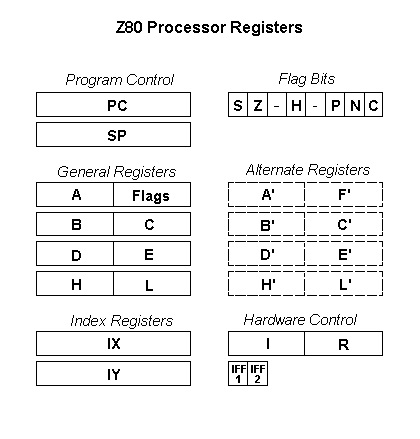
\includegraphics[width=0.5\textwidth]{images/z80registers.jpg}
    \caption{Structura registrii Z80. \cite{ref:z80registers}}
    \label{fig:z80registers}
\end{figure}

Registrul F este un registru de flaguri, acesta contine informatii despre rezultatele operatiilor aritmetice si logice.
Structura acestuia se poate vedea si in Tabela \ref{tab:z80flags}.
\begin{table}[h]
    \centering
    \begin{tabular}{|c|c|c|c|c|c|c|c|c|}
    \hline
    \textbf{Bit} & 7 & 6 & 5 & 4 & 3 & 2 & 1 & 0 \\
    \hline
    \textbf{Flag} & S & Z & F5 & H & F3 & P/V & N & C \\
    \hline
    \end{tabular}
    \caption{Z80 Flags}
    \label{tab:z80flags}
\end{table}

\subsubsection{Memorie}

Desi microprocesorul are magistrala de date pe 8 biti, acesta foloseste 16 biti pentru adresare. Datorita acestui lucru capacitatea maxima de memorie este de \(2^16=65536\) octeti, 

\subsection{Emulator}
Un emulator reprezinta o metoda hardware sau software de a imita un alt tip de sistem de calcul, cum ar fi un procesor, consola sau chiar un intreg calculator.

In cazul acestui lucrari s-a ales un emulator software, acesta fiind mult mai accesibil.

Principala aplicatie a unui emulator este de a rula un program scris pentru o anumita arhitectura pe una complet diferita.

Acest lucru ajuta in mentenanta pe termen lung permitand inlocuirea componentei hardware vechi cu una mai noua fara a necesita software nou.

In cazul curent, deoarece \ac {Z80} este destul de vechi si procurarea acestuia a devenit o problema, in cazul in care microcontrolerul necesita inlocuirea, acesta va putea fi inlocuit cu un Raspberry Pi (sau o alternativa) ruland un emulator.

%\begin{multicols}{2}

%\begin{lstlisting}[language=C++]
%#include <iostream>
%using namespace std;
%
%int main() {
%    cout << "Hello, C++!" << endl;
%    return 0;
%}
%\end{lstlisting}
%\end{multicols}

\subsection{Decizie limbaj de programare}

\section{Implementare}
This is the conclusion.

\section{Rezultate experimentale}
This is the conclusion.

\section{Contributii}
This is the conclusion.

\section{Bibliografie}
\printbibliography
\clearpage

\section{Anexe}
This is the conclusion.

\section{Planificarea activitatii}
This is the conclusion.


\end{document}
